% ----------------------------------------------------
% -------- BAYSIS - Selected as Jam Effector ---------
% ----------------------------------------------------
\subsection{Congestion - Accidents categorizes as Jam Effector}
\label{analysis_processing_correlation_baysis_effector}
The correlation matrix table for the congestion - accident dataset, which are classified as \textit{Jam Effector} (see \cref{table:appendix_correlation_matrix_matched_cramers}) is visual presented in \cref{img:correlation_matrix_selected_effector_cramers} showing the the correlation of each variable combination. When visual analyzing \cref{img:correlation_matrix_matched_cramers} and checking the guidelines for a strong correlation in reference to the applied coefficient (identifiable with \cref{table:appendix_coefficient_matrix_matched}) we get a list of strongly correlated variable combinations (see \cref{tbl:correlation_list_baysis_effector}). Since the focus of the thesis are the correlations between accidents and jams, these are only collected from the bottom-left rectangle of the matrix, where the congestion and accidents variables intersect. Correlations of the kind congestion - congestion or accident - accident are not considered.
\begin{table}[h!]
	\centering
	\begin{tabular}{c|l}  
		Category & Strong \\
		\\[-1em]
		\hline
		\\[-1em]
		Strasse & TMax, TAvg, SMax, SAvg, Cov, TLHGV \\ 
 		Kat & TMax, TAvg, SAvg \\ % + SMax % -> Strasse
 		%Typ & \\ % -> Strasse
 		%Betei & \\
 		UArt1 & SAvg \\ % -> Strasse
 		%UArt2 & \\ % -> Strasse
 		%AUrs1 & \\ % -> Strasse
 		%AUrs2 & \\
 		AufHi & TMax, TAvg \\
 		%Alkoh & \\
 		%Char1 & \\ % -> Strasse
 		%Char2 & \\ % -> Strasse
 		%Lich1 & \\ % -> Strasse
 		%Lich2 & \\ % -> Strasse
 		%Zust1 & \\ % -> Strasse
 		%Zust2 & \\ % -> Strasse
 		%Fstf & \\ % -> Strasse
 		WoTag & TAvg, SMax, Cov, TLHGV \\ % -> Strasse
 		%FeiTag & \\
 		Month & TMax, TAvg, SMax, SAvg, Cov, TLHGV \\ % -> Strasse
	\end{tabular}
    \caption{List of incident variables and their strong correlated congestion variable from the congestion-accident matched data which are classified as \textit{Jam Effector}}
	\label{tbl:correlation_list_baysis_effector}
\end{table}
Next we need to verify that the correlation is significant and what the correlation predicates. Therefore each correlation will be evaluated with the Post Hoc test, defined in \cref{correlation_posthoc}. In the following sections, the correlated relations of the variables in \cref{tbl:correlation_list_baysis_effector} are analyzed and an initial interpretation of each significant correlation is introduced. Groups with an insufficient sample size (see \cref{correlation_uncertainty} are neglected and not shown. The descriptive tables, showing the count ($n$), mean ($\bar{x}$), standard deviation ($\sigma$), median ($\tilde{x}$), $min$, $max$ and range ($\Delta$) therefore only contain groups with significant sample sizes.
\begin{figure}[!ht]
	\centering
	\makebox[\textwidth][c]{%
		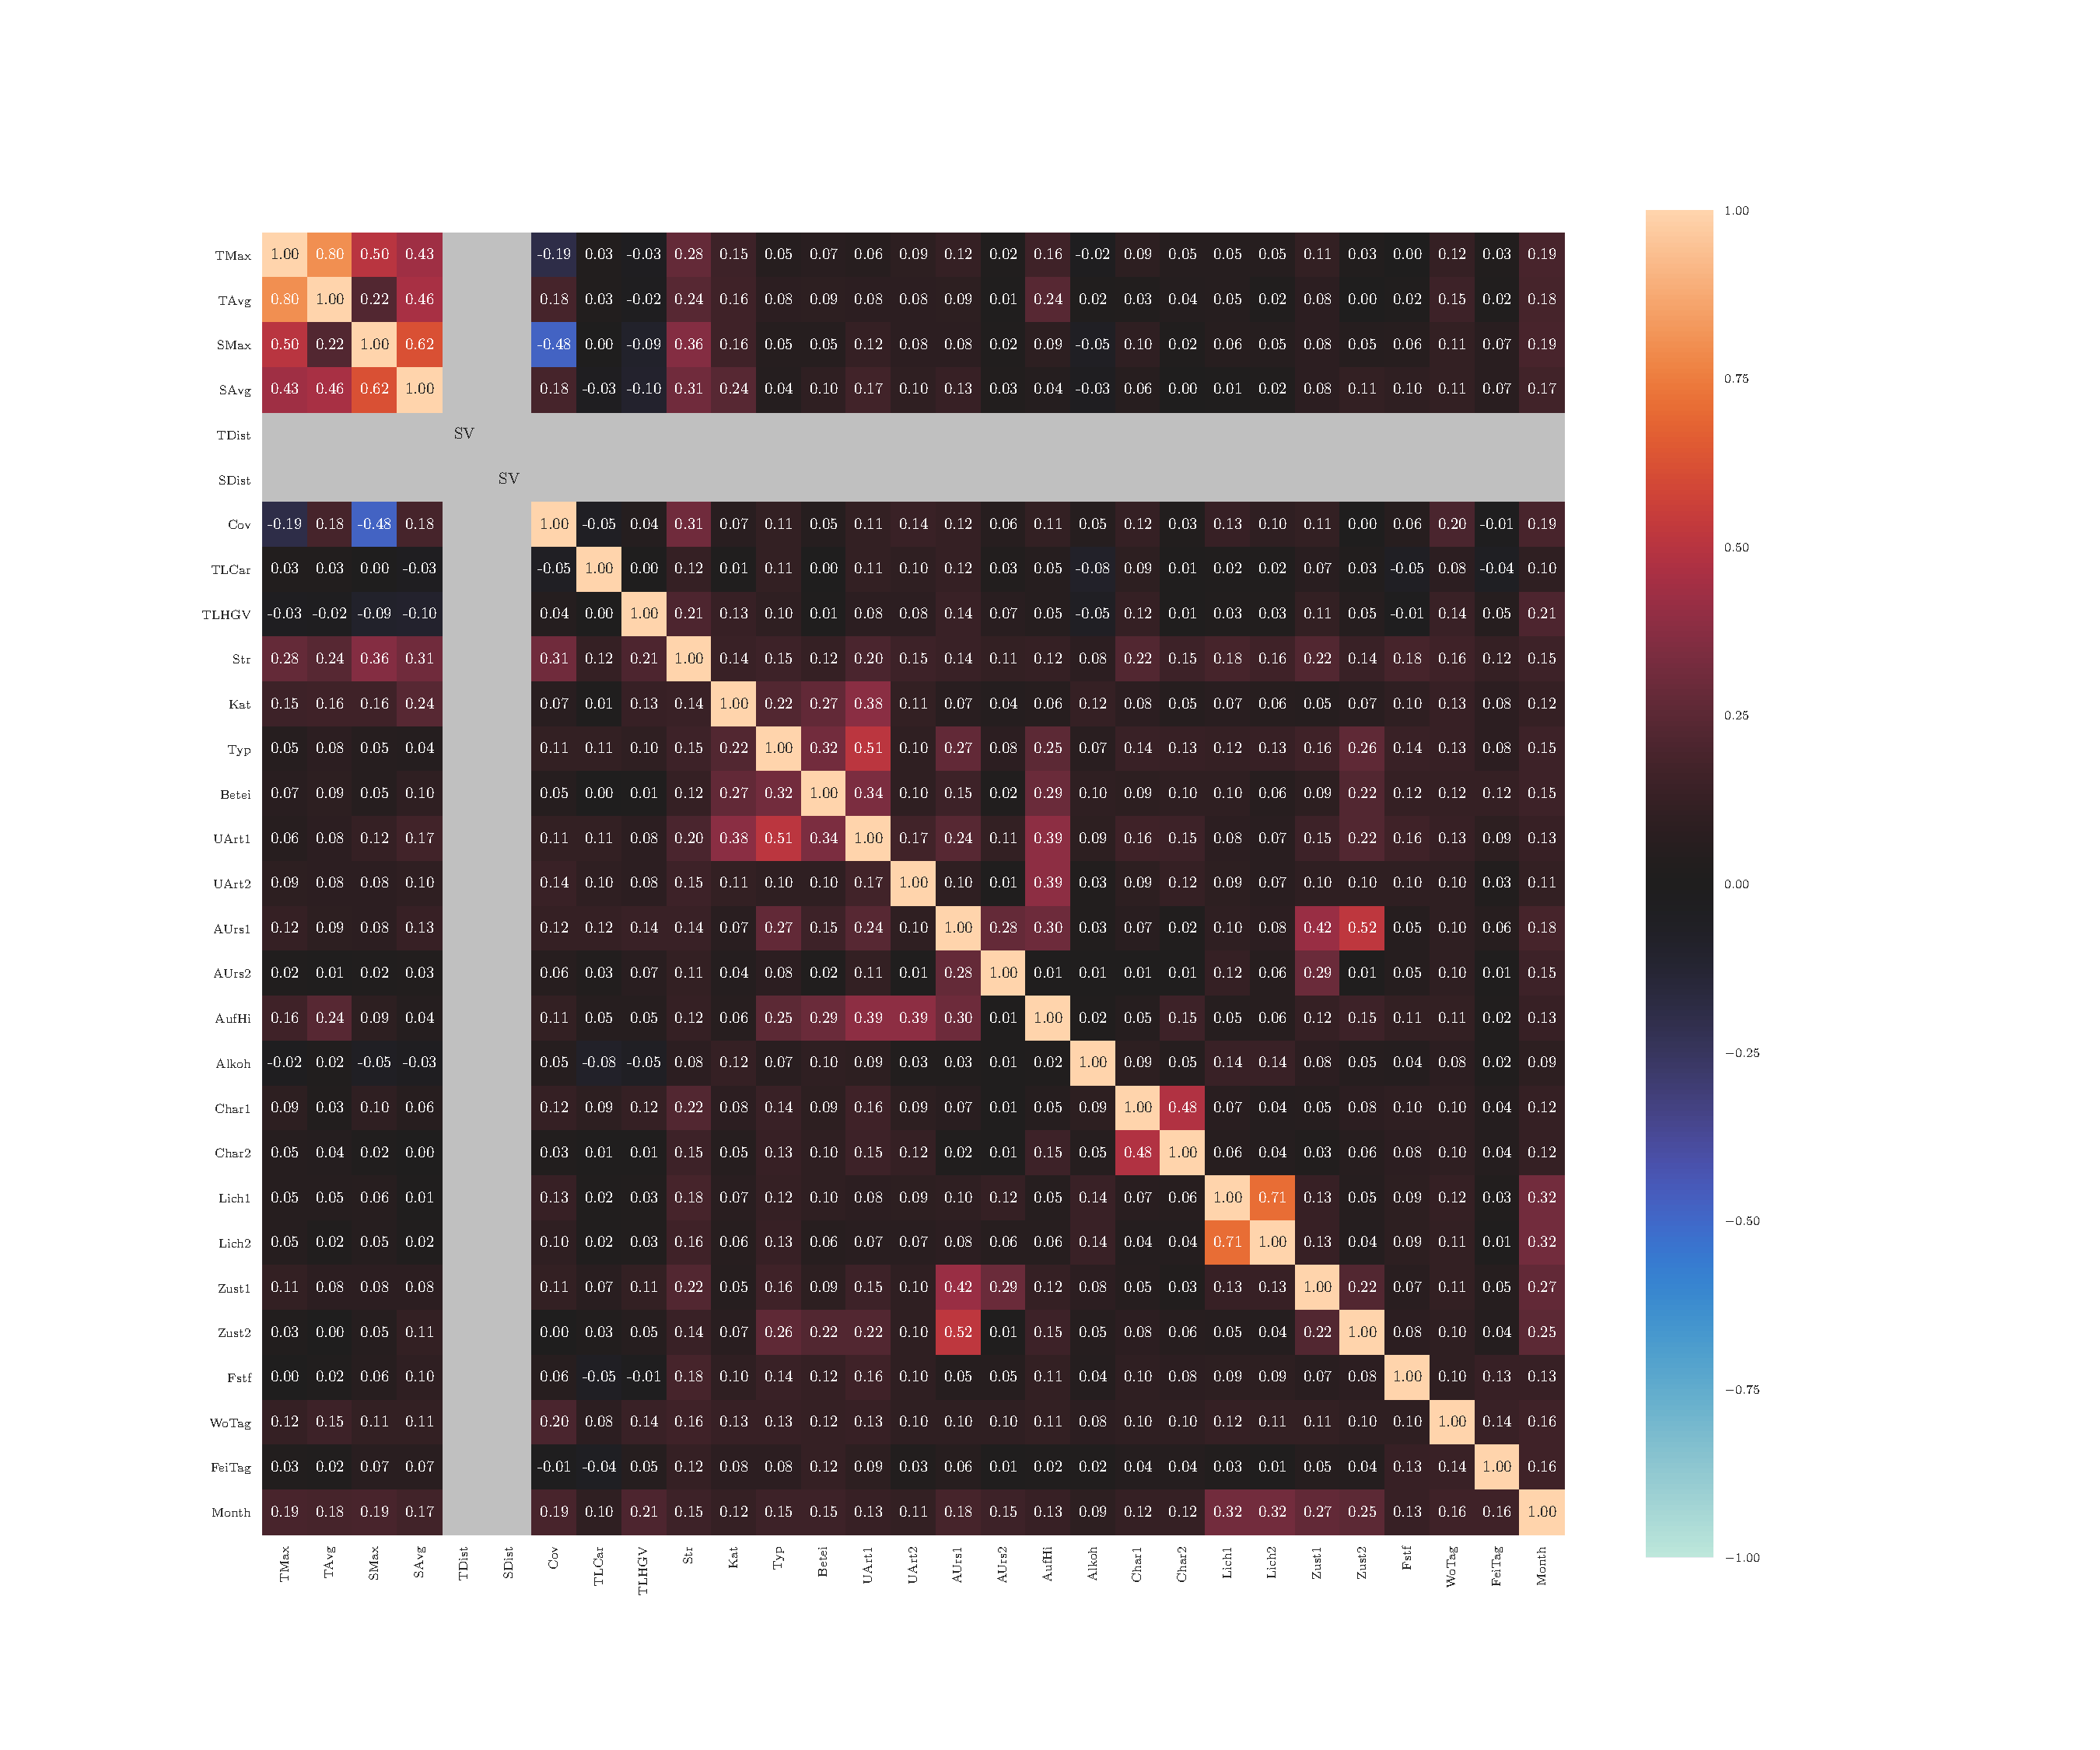
\includegraphics[width=1.4\textwidth, trim=0cm 2.5cm 6cm 3cm]{CorrAnalysis/data/BAYSIS/03_selected_02_duringJam/plots/baysis_selected_corr_cramers}%
	}
	\caption{Correlation matrix for congestion-accident matched data classified as \textit{Jam Effector} and calculated with $V$, $\eta$, $\tau$, $r_{pq}$, $r$}
	\label{img:correlation_matrix_selected_effector_cramers}
\end{figure}

% --------------------------
% -------- Strasse ---------
% --------------------------
\centerheading{Strasse}
This section analyzes the correlated relations of the accident variable \textit{Strasse}. The correlations of \textit{Strasse} - \textit{SAvg} and \textit{Strasse} - \textit{TLHGV} produces a $p$-value above the $\alpha$-level of .05 in the Kruskal-Wallis rank sum test. The null hypothesis can't therefore be rejected for these relations and there are no significant groups to identify.

The Kruskal-Wallis rank sum test of \textit{Strasse} - \textit{TMax} produces a $p$-value of 0.0104, which is below $\alpha$. The null hypothesis can therefore be rejected, which means there is a significant difference between the groups of \textit{Strasse}. To identify the significant groups, a pairwise Wilcoxon $T$-test for \textit{Strasse} - \textit{TMax} is run, which produces \cref{tbl:wilcoxon_baysis_effector_Strasse_TMax}. 
\begin{table}[ht]
	\tiny
	\centering
	\begin{tabular}{rrrrrrrrrrrrrr}
		\toprule
		     & A3 & A6 & A9 & A70 & A99 & A93 & A94 & A7 & A73 & A96 & A995 & A92 & A95 \\ 
		\midrule
		% A6   & 1.00 &  &  &  &  &  &  &  &  &  &  &  &  \\ 
		% A9   & 1.00 & 1.00 &  &  &  &  &  &  &  &  &  &  &  \\ 
		% A70  & 1.00 & 1.00 & 1.00 &  &  &  &  &  &  &  &  &  &  \\ 
		% A99  & 0.85 & 1.00 & 1.00 & 1.00 &  &  &  &  &  &  &  &  &  \\ 
		% A93  & 1.00 & 1.00 & 1.00 & 1.00 & 1.00 &  &  &  &  &  &  &  &  \\ 
		A94  & \red{0.01} & 1.00 & 0.06 & 1.00 & 0.28 & 1.00 &  &  &  &  &  &  &  \\ 
		% A7   & .00 & 1.00 & 1.00 & 1.00 & 1.00 & 1.00 & 1.00 &  &  &  &  &  &  \\ 
		A73  & \red{0.00} & 1.00 & \red{0.00} & 1.00 & 0.23 & 1.00 & 1.00 & 1.00 &  &  &  &  &  \\ 
		A96  & \red{0.00} & 1.00 & 0.35 & 1.00 & 1.00 & 1.00 & 1.00 & 1.00 & 1.00 &  &  &  &  \\ 
		% A995 & 1.00 & 1.00 & 1.00 & 1.00 & 1.00 & 1.00 & 1.00 & 1.00 & 1.00 & 1.00 &  &  &  \\ 
		A92  & \red{0.01} & 1.00 & 0.24 & 1.00 & 1.00 & 1.00 & 1.00 & 1.00 & 1.00 & 1.00 & 1.00 &  &  \\ 
		% A95  & 1.00 & 1.00 & 1.00 & 1.00 & 1.00 & 1.00 & 1.00 & 1.00 & 1.00 & 1.00 & 1.00 & 1.00 &  \\ 
		% A980 & 1.00 & 1.00 & 1.00 & 1.00 & 1.00 & 1.00 & 1.00 & 1.00 & 1.00 & 1.00 & 1.00 & 1.00 &  \\ 
		\bottomrule
	  \end{tabular}
    \caption{Pairwise Wilcoxon $T$-test for \textit{Strasse} and \textit{Maximal Temporal Extent} (Jam Effector)}
    \label{tbl:wilcoxon_baysis_effector_Strasse_TMax}
\end{table}
The table shows that the roads A94, A73, A96 and A95 differs from the A3. The A73 differs from the A9.
\begin{table}[ht]
	\tiny
	\centering
	\begin{tabular}{c|c|c|c|c|c|c|c}
		\toprule
		Group & $n$ & $\bar{x}$ & $\sigma$ & $\tilde{x}$ & $min$ & $max$ & $\Delta$ \\
		\midrule
		A3   & 265 & 297.62 & 219.09 & 243.00 & 18 & 1257 & 1239 \\ 
		A6   & 37  & 236.59 & 183.03 & 207.00 & 18 & 705  & 687  \\ 
		A9   & 192 & 243.45 & 178.97 & 201.00 & 15 & 1194 & 1179 \\ 
		A99  & 63  & 212.57 & 140.78 & 195.00 & 21 & 681  & 660  \\ 
		A93  & 12  & 212.00 & 187.74 & 130.50 & 39 & 588  & 549  \\ 
		A94  & 14  & 109.71 & 56.07  & 97.50  & 42 & 249  & 207  \\ 
		A7   & 35  & 254.66 & 306.21 & 168.00 & 42 & 1341 & 1299 \\ 
		A73  & 52  & 157.21 & 179.42 & 130.50 & 18 & 1323 & 1305 \\ 
		A96  & 41  & 155.85 & 84.33  & 144.00 & 30 & 381  & 351  \\ 
		A92  & 21  & 134.71 & 82.25  & 138.00 & 18 & 354  & 336 \\ 
		\bottomrule
	  \end{tabular}
    \caption{Group descriptives of \textit{Strasse} and \textit{Maximal Temporal Extent} (Jam Effector)}
    \label{tbl:descriptives_baysis_effector_Strasse_TMax}
	%\vspace{-8mm}
\end{table}
The descriptives from \cref{tbl:descriptives_baysis_effector_Strasse_TMax} show that the A94, A73 and A96 (the A95 is uncertain) have a mean maximal temporal distance of 140\,min. Compared to the $\bar{x}$ of the A3 of 311\,min it can be interpreted that accidents on the A3 is associated with twice as long jams than the other groups. For the A9 can be interpreted that it's accidents are associated with 40\,\% longer jams, than the A73.

The Kruskal-Wallis rank sum test of \textit{Strasse} - \textit{TAvg} produces a $p$-value of 0.0003, which is below $\alpha$. The null hypothesis can therefore be rejected, which means there is a significant difference between the groups of \textit{Strasse}. To identify the significant groups, a pairwise Wilcoxon $T$-test for \textit{Strasse} - \textit{TAvg} is run, which produces \cref{tbl:wilcoxon_baysis_effector_Strasse_TAvg}. 
\begin{table}[ht]
	\tiny
	\centering
	\begin{tabular}{rrrrrrrrrrrrrr}
		\toprule
			 & A3 & A6 & A9 & A70 & A99 & A93 & A94 & A7 & A73 & A96 & A995 & A92 & A95 \\ 
		\midrule
		% A6   & 1.00 &  &  &  &  &  &  &  &  &  &  &  &  \\ 
		% A9   & 1.00 & 1.00 &  &  &  &  &  &  &  &  &  &  &  \\ 
		% A70  & 1.00 & 1.00 & 1.00 &  &  &  &  &  &  &  &  &  &  \\ 
		A99  & \red{0.02} & 1.00 & 1.00 & 1.00 &  &  &  &  &  &  &  &  &  \\ 
		% A93  & 1.00 & 1.00 & 1.00 & 1.00 & 1.00 &  &  &  &  &  &  &  &  \\ 
		% A94  & 0.11 & 1.00 & 0.53 & 1.00 & 1.00 & 1.00 &  &  &  &  &  &  &  \\ 
		% A7   & 1.00 & 1.00 & 1.00 & 1.00 & 1.00 & 1.00 & 0.61 &  &  &  &  &  &  \\ 
		A73  & \red{0.00} & 1.00 & 0.00 & 1.00 & 1.00 & 1.00 & 1.00 & \red{0.02} &  &  &  &  &  \\ 
		% A96  & 1.00 & 1.00 & 1.00 & 1.00 & 1.00 & 1.00 & 1.00 & 1.00 & 0.87 &  &  &  &  \\ 
		% A995 & 1.00 & 1.00 & 1.00 & 1.00 & 1.00 & 1.00 & 1.00 & 1.00 & 1.00 & 1.00 &  &  &  \\ 
		% A92  & 1.00 & 1.00 & 1.00 & 1.00 & 1.00 & 1.00 & 1.00 & 1.00 & 1.00 & 1.00 & 1.00 &  &  \\ 
		% A95  & 1.00 & 1.00 & 1.00 & 1.00 & 1.00 & 1.00 & 1.00 & 1.00 & 1.00 & 1.00 & 1.00 & 1.00 &  \\ 
		% A980 & 1.00 & 1.00 & 1.00 & 1.00 & 1.00 & 1.00 & 1.00 & 1.00 & 1.00 & 1.00 & 1.00 & 1.00 & 1.00 \\ 
		\bottomrule
	  \end{tabular}
    \caption{Pairwise Wilcoxon $T$-test for \textit{Strasse} and \textit{Average Temporal Extent} (Jam Effector)}
    \label{tbl:wilcoxon_baysis_effector_Strasse_TAvg}
\end{table}
The table shows that the roads A99 and A73 differ from the A3. The A73 also differs from A7.
\begin{table}[ht]
	\tiny
	\centering
	\begin{tabular}{c|c|c|c|c|c|c|c}
		\toprule
		Group & $n$ & $\bar{x}$ & $\sigma$ & $\tilde{x}$ & $min$ & $max$ & $\Delta$ \\
		\midrule
		A3   & 265 & 104.05 & 87.02 & 84.00 & 7  & 703  & 696 \\ 
		A6   & 37  & 82.43  & 74.19  & 70.00 & 3  & 301  & 298 \\ 
		A9   & 192 & 91.31  & 74.64  & 75.00 & 5  & 575  & 570 \\  
		A99  & 63  & 65.73  & 47.32  & 52.00 & 4  & 295  & 291 \\ 
		A93  & 12  & 104.83 & 112.03 & 55.00 & 7  & 343  & 336 \\ 
		A94  & 14  & 45.93  & 25.54  & 43.00 & 14 & 102  & 88 \\ 
		A7   & 35  & 143.74 & 255.78 & 76.00 & 15 & 1326 & 1311 \\ 
		A73  & 52  & 47.63  & 29.09  & 44.00 & 6  & 154  & 148 \\ 
		A96  & 41  & 74.39  & 54.53  & 70.00 & 6  & 247  & 241 \\ 
		A92  & 21  & 64.52  & 48.86  & 56.00 & 8  & 235  & 227 \\ 
		\bottomrule
	  \end{tabular}
    \caption{Group descriptives of \textit{Strasse} and \textit{Average Temporal Extent} (Jam Effector)}
    \label{tbl:descriptives_baysis_effector_Strasse_TAvg}
	%\vspace{-8mm}
\end{table}
The descriptives in \cref{tbl:descriptives_baysis_effector_Strasse_TAvg} show that the mean $\bar{x}$ of the groups A99 and A73 is 56\,min, which is nearly 50\,\% lower than the $\bar{x}$ of A3. The $\bar{x}$ of A73 is also just $\frac{1}{3}$ compared to the A94. It can be interpreted that accidents on the A3 and A7 are associated with significantly longer jams than on other roads.

The Kruskal-Wallis rank sum test of \textit{Strasse} - \textit{SMax} produces a $p$-value of 0.0025, which is below $\alpha$. The null hypothesis can therefore be rejected, which means there is a significant difference between the groups of \textit{Strasse}. To identify the significant groups, a pairwise Wilcoxon $T$-test for \textit{Strasse} - \textit{SMax} is run, which produces \cref{tbl:wilcoxon_baysis_effector_Strasse_SMax}. 
\begin{table}[ht]
	\tiny
	\centering
	\begin{tabular}{rrrrrrrrrrrrrr}
		\toprule
			 & A3 & A6 & A9 & A70 & A99 & A93 & A94 & A7 & A73 & A96 & A995 & A92 & A95 \\ 
		\midrule
		% A6   & 1.00 &  &  &  &  &  &  &  &  &  &  &  &  \\ 
		A9   & \red{0.00} & 1.00 &  &  &  &  &  &  &  &  &  &  &  \\ 
		% A70  & 1.00 & 1.00 & 1.00 &  &  &  &  &  &  &  &  &  &  \\ 
		% A99  & 1.00 & 1.00 & 1.00 & 1.00 &  &  &  &  &  &  &  &  &  \\ 
		A93  & 0.07 & 0.13 & 1.00 & 1.00 & 1.00 &  &  &  &  &  &  &  &  \\ 
		A94  & \red{0.01} & \red{0.03} & 0.41 & 1.00 & 0.24 & 1.00 &  &  &  &  &  &  &  \\ 
		A7   & 0.08 & 0.65 & 1.00 & 1.00 & 1.00 & 1.00 & 1.00 &  &  &  &  &  &  \\ 
		A73  & \red{0.00} & \red{0.00} & \red{0.00} & 1.00 & \red{0.00} & 1.00 & 1.00 & 0.95 &  &  &  &  &  \\ 
		A96  & 0.13 & 1.00 & 1.00 & 1.00 & 1.00 & 1.00 & 1.00 & 1.00 & 0.18 &  &  &  &  \\ 
		% A995 & 1.00 & 1.00 & 1.00 & 1.00 & 1.00 & 1.00 & 1.00 & 1.00 & 1.00 & 1.00 &  &  &  \\ 
		A92  & \red{0.00} & \red{0.00} & \red{0.04} & 1.00 & \red{0.04} & 1.00 & 1.00 & 1.00 & 1.00 & 1.00 & 1.00 &  &  \\ 
		% A95  & 1.00 & 1.00 & 1.00 & 1.00 & 1.00 & 1.00 & 1.00 & 1.00 & 1.00 & 1.00 & 1.00 & 1.00 &  \\ 
		% A980 & 1.00 & 1.00 & 1.00 & 1.00 & 1.00 & 1.00 & 1.00 & 1.00 & 1.00 & 1.00 & 1.00 & 1.00 & 1.00 \\ 
		\bottomrule
	  \end{tabular}
    \caption{Pairwise Wilcoxon $T$-test for \textit{Strasse} and \textit{Maximal Spatial Extent} (Jam Effector)}
    \label{tbl:wilcoxon_baysis_effector_Strasse_SMax}
\end{table}
The table shows that the roads of A9, A73, and A92 differ significantly from A3. The roads A94, A73 and A92 also differ significantly from A6. A73 and A92 also differ significantly from A9 and A99, but there is no distinctive trend.
\begin{table}[ht]
	\tiny
	\centering
	\begin{tabular}{c|c|c|c|c|c|c|c}
		\toprule
		Group & $n$ & $\bar{x}$ & $\sigma$ & $\tilde{x}$ & $min$ & $max$ & $\Delta$ \\
		\midrule
		A3   & 265 & 17755.15 & 11139.22 & 14811.00 & 1566 & 46328 & 44762 \\ 
		A6   & 37  & 16711.43 & 9518.81  & 14449.00 & 2655 & 40033 & 37378 \\ 
		A9   & 192 & 13271.42 & 8473.71  & 11654.50 & 1315 & 49765 & 48450 \\ 
		A99  & 63  & 17558.70 & 12223.42 & 14698.00 & 2351 & 48278 & 45927 \\ 
		A93  & 12  & 8158.42  & 4473.23  & 7461.50  & 2896 & 16922 & 14026 \\ 
		A94  & 14  & 7277.64  & 4218.45  & 6947.00  & 1206 & 15550 & 14344 \\ 
		A7   & 35  & 11825.00 & 8885.99  & 9506.00  & 3041 & 43244 & 40203 \\ 
		A73  & 52  & 7964.98  & 5995.59  & 6559.50  & 1036 & 33764 & 32728 \\ 
		A96  & 41  & 11825.98 & 6911.19  & 9676.00  & 2006 & 27965 & 25959 \\ 
		A92  & 21  & 7255.76  & 3637.71  & 7364.00  & 1176 & 13522 & 12346 \\ 
		\bottomrul
	  \end{tabular}
    \caption{Group descriptives of \textit{Strasse} and \textit{Maximal Spatial Extent} (Jam Effector)}
    \label{tbl:descriptives_baysis_effector_Strasse_SMax}
	%\vspace{-8mm}
\end{table}
The descriptives in \cref{tbl:descriptives_baysis_effector_Strasse_SMax} show that $\bar{x}$ of A6, A7, A9, A96 and A99 are between 50\,\% to 80\,\% higher than A73, A92, A93 and A94. The $\bar{x}$ of A3 supersedes the A6, A7, A9, A96 and A99 by a similar amount again. It can be interpreted that the maximal spatial distance varies from A73, A92, A93 and A94 over A6, A7, A9, A96 and A99 to the A3, by up to 340\,\%.

The Kruskal-Wallis rank sum test of \textit{Strasse} - \textit{Cov} produces a $p$-value of 0.0055, which is below $\alpha=.05$. The null hypothesis can therefore be rejected, which means there is a significant difference between the groups of \textit{Strasse}. To identify the significant groups, a pairwise Wilcoxon $T$-test for \textit{Strasse} - \textit{Cov} is run, which produces \cref{tbl:wilcoxon_baysis_effector_Strasse_Cov}. 
\begin{table}[ht]
	\tiny
	\centering
	\begin{tabular}{rrrrrrrrrrrrrr}
		\toprule
			 & A3 & A6 & A9 & A70 & A99 & A93 & A94 & A7 & A73 & A96 & A995 & A92 & A95 \\ 
		\midrule
		% A6   & 1.00 &  &  &  &  &  &  &  &  &  &  &  &  \\ 
		A9   & \red{0.01} & 1.00 &  &  &  &  &  &  &  &  &  &  &  \\ 
		% A70  & 1.00 & 1.00 & 1.00 &  &  &  &  &  &  &  &  &  &  \\ 
		A99  & 1.00 & 1.00 & \red{0.00} & 1.00 &  &  &  &  &  &  &  &  &  \\ 
		% A93  & 1.00 & 1.00 & 1.00 & 1.00 & 1.00 &  &  &  &  &  &  &  &  \\ 
		% A94  & 1.00 & 1.00 & 1.00 & 1.00 & 1.00 & 1.00 &  &  &  &  &  &  &  \\ 
		A7   & 0.25 & 1.00 & 1.00 & 1.00 & \red{0.02} & 1.00 & 1.00 &  &  &  &  &  &  \\ 
		% A73  & 1.00 & 1.00 & 1.00 & 1.00 & 1.00 & 1.00 & 1.00 & 1.00 &  &  &  &  &  \\ 
		A96  & 0.21 & 1.00 & 1.00 & 1.00 & \red{0.02} & 1.00 & 1.00 & 1.00 & 1.00 &  &  &  &  \\ 
		% A995 & 1.00 & 1.00 & 1.00 & 1.00 & 1.00 & 1.00 & 1.00 & 1.00 & 1.00 & 1.00 &  &  &  \\ 
		A92  & \red{0.03} & 0.43 & 1.00 & 1.00 & \red{0.01} & 1.00 & 1.00 & 1.00 & 0.61 & 1.00 & 1.00 &  &  \\ 
		% A95  & 1.00 & 1.00 & 1.00 & 1.00 & 1.00 & 1.00 & 1.00 & 1.00 & 1.00 & 1.00 & 1.00 & 1.00 &  \\ 
		% A980 & 1.00 & 1.00 & 1.00 & 1.00 & 1.00 & 1.00 & 1.00 & 1.00 & 1.00 & 1.00 & 1.00 & 1.00 & 1.00 \\ 
		\bottomrule
	  \end{tabular}
    \caption{Pairwise Wilcoxon $T$-test for \textit{Strasse} and \textit{Coverage} (Jam Effector)}
    \label{tbl:wilcoxon_baysis_effector_Strasse_Cov}
\end{table}
The table shows that roads A9 and A92 differ significantly from A3. The road A99 differs significantly A9. The roads A7, A96 and A92 differ significantly from A99.
\begin{table}[ht]
	\tiny
	\centering
	\begin{tabular}{c|c|c|c|c|c|c|c}
		\toprule
		Group & $n$ & $\bar{x}$ & $\sigma$ & $\tilde{x}$ & $min$ & $max$ & $\Delta$ \\
		\midrule
		A3   & 265 & 32.02 & 16.40 & 28.0 & 2  & 100 & 92 \\ 
		A6   & 37  & 30.81 & 16.61 & 25.0 & 9  & 65  & 56 \\ 
		A9   & 192 & 36.09 & 13.77 & 34.5 & 6  & 86  & 80 \\ 
		A99  & 63  & 26.79 & 14.71 & 25.0 & 7  & 63  & 56 \\ 
		A93  & 12  & 37.25 & 17.78 & 36.5 & 13 & 70  & 57 \\ 
		A94  & 14  & 36.79 & 21.00 & 33.5 & 11 & 77  & 66 \\ 
		A7   & 35  & 45.60 & 25.54 & 42.0 & 6  & 100 & 94 \\ 
		A73  & 52  & 32.94 & 15.73 & 30.5 & 7  & 77  & 70 \\ 
		A96  & 41  & 42.90 & 21.63 & 42.0 & 9  & 85  & 76 \\ 
		A92  & 21  & 47.71 & 22.04 & 47.0 & 21 & 88  & 67 \\ 
		\bottomrule
	  \end{tabular}
    \caption{Group descriptives of \textit{Strasse} and \textit{Coverage} (Jam Effector)}
    \label{tbl:descriptives_baysis_effector_Strasse_Cov}
	%\vspace{-8mm}
\end{table}
The descriptives in \cref{tbl:descriptives_baysis_effector_Strasse_Cov} show that the $\bar{x}$ of A9 and A92 is 20\,\% and 56\,\% higher than A3. The $\bar{x}$ of A99 is the lower and 38\,\% lower than A9. A7, A96 and A92 have the highest $\bar{x}$ with 73\,\%, 61\,\% and 80\,\% above A99. It can be interpreted that the coverage increases from A3 over A9 and A92 to A7, A96 and A92 by up to 80\,\%.

\clearpage

% ----------------------
% -------- Kat ---------
% ----------------------
\centerheading{Kat}
The relations of \textit{Kat} - \textit{TMax}, \textit{Kat} - \textit{TAvg} and \textit{Kat} - \textit{SAvg} produce a $p$-value above the $\alpha$-level. The null hypothesizes can't be rejected and there are no significant differences between the groups of \textit{Kat}. There are no significant groups to identify.

% ------------------------
% -------- UArt1 ---------
% ------------------------
\centerheading{UArt}
The relation of \textit{UArt1} - \textit{SAvg} produces a $p$-value above the $\alpha$-level. The null hypothesizes can't be rejected and there are no significant differences between the groups of \textit{UArt1} and \textit{UArt2}. There are no significant groups to identify.

% ------------------------
% -------- AufHi ---------
% ------------------------
\centerheading{AufHi}
Both relations \textit{AufHi} - \textit{TMax} and \textit{AufHi} - \textit{TAvg} produce a $p$-value above the $\alpha$-level in the Kruskal-Wallis rank sum test. The null hypothesizes can't be rejected and there are no significant differences between the groups of \textit{AufHi}. There are therefore no significant groups to identify.

% ------------------------
% -------- WoTag ---------
% ------------------------
\centerheading{WoTag}
This section analyzes the correlated relations of the accident variable \textit{WoTag}. The Kruskal-Wallis rank sum test of \textit{WoTag} - \textit{TAvg} and \textit{WoTag} - \textit{Cov} produce a $p$-value above $\alpha=.05$. The null hypothesis for these relations can't be rejected and there is no significant difference between the groups of \textit{WoTag} in regards of \textit{TAvg} and \textit{Cov}.

The Kruskal-Wallis rank sum test of \textit{WoTag} - \textit{SMax} produces a $p$-value of 0.0175, which is below $\alpha$. The null hypothesis can therefore be rejected, which means there is a significant difference between the groups of \textit{WoTag}. To identify the significant groups, a pairwise Wilcoxon $T$-test for \textit{WoTag} - \textit{SMax} is run, which produces \cref{tbl:wilcoxon_baysis_effector_WoTag_TMax}. 
\begin{table}[ht!]
	\tiny
	\centering
	\begin{tabular}{rrrrrrr}
		\toprule
		   & Di & Do & Fr & Mi & Mo & Sa \\ 
		\midrule
		Do & 1.00 &  &  &  &  &  \\ 
		Fr & 1.00 & 1.00 &  &  &  &  \\ 
		Mi & 1.00 & 1.00 & 1.00 &  &  &  \\ 
		Mo & 1.00 & 1.00 & 1.00 & 1.00 &  &  \\ 
		Sa & 1.00 & 1.00 & 1.00 & 1.00 & 1.00 &  \\ 
		So & 1.00 & 1.00 & 1.00 & 1.00 & 1.00 & 1.00 \\ 
		\bottomrule
	  \end{tabular}
    \caption{Pairwise Wilcoxon $T$-test for \textit{WoTag} and \textit{Maximal Spatial Extent}}
    \label{tbl:wilcoxon_baysis_effector_WoTag_TMax}
\end{table}
The tables shows that the differences are not group specific, which means that the relation can be neglected (see \cref{correlation_posthoc}).

The Kruskal-Wallis rank sum test of \textit{WoTag} - \textit{TLHGV} produces a $p$-value of 0.0089, which is below $\alpha$. The null hypothesis can therefore be rejected, which means there is a significant difference between the groups of \textit{WoTag}. To identify the significant groups, a pairwise Wilcoxon $T$-test for \textit{WoTag} - \textit{TLHGV} is run, which produces \cref{tbl:wilcoxon_baysis_effector_WoTag_TLHGV}. 
\begin{table}[ht!]
	\tiny
	\centering
    \begin{tabular}{rrrrrrr}
		\toprule
		   & Di & Do & Fr & Mi & Mo & Sa \\ 
		\midrule
		% Do & 1.00 &  &  &  &  &  \\ 
		% Fr & 1.00 & 1.00 &  &  &  &  \\ 
		Mi & \red{0.03} & 1.00 & 1.00 &  &  &  \\ 
		% Mo & 0.82 & 1.00 & 1.00 & 1.00 &  &  \\ 
		% Sa & 1.00 & 1.00 & 1.00 & 0.82 & 1.00 &  \\ 
		So & 1.00 & 1.00 & 1.00 & \red{0.05} & 0.65 & 1.00 \\ 
		\bottomrule
	\end{tabular}
    \caption{Pairwise Wilcoxon $T$-test for \textit{WoTag} and \textit{Time-loss HGV}}
    \label{tbl:wilcoxon_baysis_effector_WoTag_TLHGV}
\end{table}
\todo{Explain}
\begin{table}[ht!]
	\tiny
	\centering
    \begin{tabular}{c|c|c|c|c|c|c|c}
		\toprule
		Group & $n$ & $\bar{x}$ & $\sigma$ & $\tilde{x}$ & $min$ & $max$ & $\Delta$ \\
		\midrule
		Di & 115 & 766.97 & 141.79 & 794.00 & 518 & 999 & 481 \\ 
		Do & 129 & 739.48 & 143.28 & 720.00 & 511 & 983 & 472 \\ 
		Fr & 142 & 739.78 & 155.44 & 720.00 & 502 & 998 & 496 \\ 
		Mi & 124 & 709.44 & 140.31 & 692.50 & 501 & 995 & 494 \\ 
		Mo & 89  & 728.10 & 134.08 & 727.00 & 514 & 986 & 472 \\ 
		Sa & 65  & 750.46 & 143.80 & 778.00 & 507 & 988 & 481 \\ 
		So & 73  & 774.67 & 141.34 & 784.00 & 534 & 994 & 460 \\ 
		\bottomrule
	\end{tabular}
    \caption{Group descriptives of \textit{WoTag} and \textit{Time-loss HGV}}
    \label{tbl:descriptives_baysis_effector_WoTag_TLHGV}
	%\vspace{-8mm}
\end{table}

% ------------------------
% -------- Month ---------
% ------------------------
\centerheading{Month}
This section analyzes the correlated relations of the accident variable \textit{Month}. The Kruskal-Wallis rank sum test of \textit{Month} - \textit{TMax}, \textit{Month} - \textit{TAvg}, \textit{Month} - \textit{TLHGV} and \textit{Month} - \textit{Cov} produce a $p$-value above the $\alpha$-level. The null hypothesis for these relations can't be rejected and there is no significant difference between the groups of \textit{Month} in regards of \textit{TMax}, \textit{TAvg}, \textit{TLHGV} and \textit{Cov}.
% \paragraph{Maximal Temporal Extent}
% Kruskal-Wallis chi-squared = 197.96, df = 199, p-value = 0.5074

\begin{table}[ht]
	\tiny
	\centering
	\begin{tabular}{rrrrrrrrrrrr}
		\toprule
		& 0 & 1 & 2 & 3 & 4 & 5 & 6 & 7 & 8 & 9 & 10 \\ 
		\midrule
		1 & 1.00 &  &  &  &  &  &  &  &  &  &  \\ 
		2 & 1.00 & 1.00 &  &  &  &  &  &  &  &  &  \\ 
		3 & 1.00 & 1.00 & 1.00 &  &  &  &  &  &  &  &  \\ 
		4 & 1.00 & 1.00 & 1.00 & 1.00 &  &  &  &  &  &  &  \\ 
		5 & 1.00 & 1.00 & 1.00 & 1.00 & 1.00 &  &  &  &  &  &  \\ 
		6 & 1.00 & 1.00 & 0.35 & 1.00 & 1.00 & 1.00 &  &  &  &  &  \\ 
		7 & 1.00 & 1.00 & 1.00 & 1.00 & 1.00 & 1.00 & 1.00 &  &  &  &  \\ 
		8 & 1.00 & 1.00 & 0.62 & 1.00 & 1.00 & 1.00 & 1.00 & 1.00 &  &  &  \\ 
		9 & 1.00 & 1.00 & 1.00 & 1.00 & 1.00 & 1.00 & 0.20 & 1.00 & 0.40 &  &  \\ 
		10 & 1.00 & 1.00 & 1.00 & 1.00 & 1.00 & 0.38 & 0.00 & 0.09 & 0.01 & 1.00 &  \\ 
		11 & 1.00 & 1.00 & 1.00 & 1.00 & 1.00 & 1.00 & 1.00 & 1.00 & 1.00 & 1.00 & 0.91 \\ 
		\bottomrule
	\end{tabular}
    \caption{Pairwise Wilcoxon $T$-test for \textit{Month} and \textit{Maximal Spatial Extent}}
    \label{tbl:wilcoxon_baysis_effector_AUrs1_Cov}
\end{table}
\todo{Explain}
\begin{table}[ht]
	\tiny
	\centering
	\begin{tabular}{rrrrrrrrrrrrrr}
		\toprule
		& vars & n & mean & sd & median & trimmed & mad & min & max & range & skew & kurtosis & se \\ 
		\midrule
		X1   & 1.00 & 39.00 & 15204.44 & 10633.53 & 11151.00 & 14423.06 & 8507.16 & 1772.00 & 38867.00 & 37095.00 & 0.72 & -0.79 & 1702.73 \\ 
		X11  & 1.00 & 38.00 & 13921.39 & 9612.90 & 12118.50 & 12777.91 & 9202.50 & 1176.00 & 44548.00 & 43372.00 & 1.20 & 1.53 & 1559.42 \\ 
		X12  & 1.00 & 51.00 & 12295.18 & 9266.62 & 9669.00 & 11234.27 & 8197.30 & 1206.00 & 48278.00 & 47072.00 & 1.34 & 2.47 & 1297.59 \\ 
		X13  & 1.00 & 57.00 & 15190.47 & 11402.17 & 12433.00 & 13719.66 & 10090.58 & 1415.00 & 43070.00 & 41655.00 & 1.07 & 0.24 & 1510.25 \\ 
		X14  & 1.00 & 53.00 & 25006.21 & 48825.44 & 12057.00 & 13576.56 & 9733.27 & 1315.00 & 219082.00 & 217767.00 & 3.52 & 11.14 & 6706.69 \\ 
		X15  & 1.00 & 60.00 & 25007.18 & 45097.00 & 12339.00 & 13513.90 & 8289.96 & 2632.00 & 189730.00 & 187098.00 & 3.21 & 8.88 & 5822.00 \\ 
		X16  & 1.00 & 114.00 & 17771.96 & 12364.77 & 14791.00 & 16233.34 & 9751.06 & 1036.00 & 64943.00 & 63907.00 & 1.20 & 1.28 & 1158.07 \\ 
		X17  & 1.00 & 90.00 & 18327.20 & 28345.23 & 11955.00 & 13190.35 & 6828.11 & 2500.00 & 195310.00 & 192810.00 & 5.41 & 30.81 & 2987.85 \\ 
		X18  & 1.00 & 83.00 & 18134.89 & 16807.92 & 16198.00 & 15904.31 & 9974.93 & 2006.00 & 135780.00 & 133774.00 & 4.25 & 26.34 & 1844.91 \\ 
		X19  & 1.00 & 65.00 & 14558.85 & 19682.16 & 9917.00 & 11682.72 & 8178.02 & 1524.00 & 153237.00 & 151713.00 & 5.41 & 35.02 & 2441.27 \\ 
		X110 & 1.00 & 56.00 & 10844.89 & 8940.48 & 8712.00 & 9417.35 & 6484.15 & 1883.00 & 36151.00 & 34268.00 & 1.40 & 1.15 & 1194.72 \\ 
		X111 & 1.00 & 49.00 & 15302.61 & 11066.27 & 11386.00 & 14171.83 & 7064.59 & 1925.00 & 43244.00 & 41319.00 & 1.02 & -0.06 & 1580.90 \\ 
		\bottomrule
	\end{tabular}
    \caption{Group descriptives of \textit{Month} and \textit{Maximal Spatial Extent}}
    \label{tbl:descriptives_baysis_effector_AUrs1_Cov}
	%\vspace{-8mm}
\end{table}

\paragraph{Average Spatial Extent}
Kruskal-Wallis chi-squared = 719.2, df = 647, p-value = 0.02528

\begin{table}[ht]
	\tiny
	\centering
	\begin{tabular}{rrrrrrrrrrrr}
		\toprule
		& 0 & 1 & 2 & 3 & 4 & 5 & 6 & 7 & 8 & 9 & 10 \\ 
		\midrule
		1  & 1.00 &  &  &  &  &  &  &  &  &  &  \\ 
		2  & 1.00 & 1.00 &  &  &  &  &  &  &  &  &  \\ 
		3  & 1.00 & 1.00 & 1.00 &  &  &  &  &  &  &  &  \\ 
		4  & 1.00 & 1.00 & 1.00 & 1.00 &  &  &  &  &  &  &  \\ 
		5  & 1.00 & 1.00 & 1.00 & 1.00 & 1.00 &  &  &  &  &  &  \\ 
		6  & 1.00 & 1.00 & 1.00 & 1.00 & 1.00 & 1.00 &  &  &  &  &  \\ 
		7  & 1.00 & 1.00 & 1.00 & 1.00 & 1.00 & 1.00 & 1.00 &  &  &  &  \\ 
		8  & 1.00 & 1.00 & 0.77 & 1.00 & 1.00 & 1.00 & 1.00 & 1.00 &  &  &  \\ 
		9  & 1.00 & 1.00 & 1.00 & 1.00 & 1.00 & 1.00 & 1.00 & 1.00 & 1.00 &  &  \\ 
		10 & 1.00 & 1.00 & 1.00 & 1.00 & 1.00 & 1.00 & 0.58 & 1.00 & 0.07 & 1.00 &  \\ 
		11 & 1.00 & 1.00 & 0.33 & 1.00 & 1.00 & 1.00 & 1.00 & 1.00 & 1.00 & 1.00 & 0.07 \\ 
		\bottomrule
	  \end{tabular}
    \caption{Pairwise Wilcoxon $T$-test for \textit{Month} and \textit{Average Spatial Extent}}
    \label{tbl:wilcoxon_baysis_effector_AUrs1_Cov}
\end{table}
\todo{Explain}
\begin{table}[ht]
	\tiny
	\centering
	\begin{tabular}{rrrrrrrrrrrrrr}
		\toprule
		& vars & n & mean & sd & median & trimmed & mad & min & max & range & skew & kurtosis & se \\ 
		\midrule
		X1   & 1.00 & 39.00 & 4600.31 & 3223.30 & 4111.00 & 4160.21 & 2573.79 & 829.00 & 14785.00 & 13956.00 & 1.41 & 1.62 & 516.14 \\ 
		X11  & 1.00 & 38.00 & 4046.26 & 2217.96 & 3833.50 & 3957.81 & 2490.77 & 853.00 & 8426.00 & 7573.00 & 0.37 & -1.10 & 359.80 \\ 
		X12  & 1.00 & 51.00 & 3803.96 & 2410.63 & 2944.00 & 3592.93 & 2440.36 & 747.00 & 10494.00 & 9747.00 & 0.64 & -0.49 & 337.56 \\ 
		X13  & 1.00 & 57.00 & 3990.09 & 2120.45 & 3865.00 & 3832.34 & 2301.00 & 670.00 & 10320.00 & 9650.00 & 0.64 & 0.17 & 280.86 \\ 
		X14  & 1.00 & 53.00 & 4248.15 & 2616.85 & 3916.00 & 4054.23 & 3168.32 & 393.00 & 10614.00 & 10221.00 & 0.53 & -0.75 & 359.45 \\ 
		X15  & 1.00 & 60.00 & 4670.23 & 2895.41 & 3942.00 & 4385.75 & 2641.25 & 779.00 & 11206.00 & 10427.00 & 0.77 & -0.53 & 373.80 \\ 
		X16  & 1.00 & 114.00 & 4491.17 & 2627.83 & 3835.00 & 4220.82 & 2221.68 & 784.00 & 15132.00 & 14348.00 & 1.27 & 2.28 & 246.12 \\ 
		X17  & 1.00 & 90.00 & 4379.04 & 2574.30 & 3625.50 & 4084.78 & 2092.69 & 1036.00 & 13744.00 & 12708.00 & 1.06 & 0.81 & 271.35 \\ 
		X18  & 1.00 & 83.00 & 4921.23 & 2760.05 & 4251.00 & 4616.57 & 2630.13 & 786.00 & 13605.00 & 12819.00 & 1.01 & 0.72 & 302.95 \\ 
		X19  & 1.00 & 65.00 & 4054.97 & 2206.33 & 3953.00 & 3975.55 & 2581.21 & 358.00 & 8116.00 & 7758.00 & 0.31 & -1.00 & 273.66 \\ 
		X110 & 1.00 & 56.00 & 3591.02 & 2391.39 & 2976.50 & 3246.24 & 1956.29 & 660.00 & 11167.00 & 10507.00 & 1.36 & 1.50 & 319.56 \\ 
		X111 & 1.00 & 49.00 & 5380.88 & 3286.83 & 4804.00 & 5069.46 & 3089.74 & 1006.00 & 17805.00 & 16799.00 & 1.32 & 2.76 & 469.55 \\ 
		\bottomrule
	\end{tabular}
    \caption{Group descriptives of \textit{Month} and \textit{Average Spatial Extent}}
    \label{tbl:descriptives_baysis_effector_AUrs1_Cov}
	%\vspace{-8mm}
\end{table}